\documentclass[12pt]{llncs}
                   

\usepackage {mathpartir}
\usepackage{bcprules}
%\usepackage{listings}
                       
\usepackage{graphicx} 
%\usepackage[margins=2.5cm,nohead,nofoot]{geometry}
\usepackage{geometry}
\usepackage{amsfonts}
\usepackage{amstext}
\usepackage{latexsym}
\usepackage{amssymb}


%\include{myPreamble}

% Double brackets
\newcommand{\ldb}{[\![}
\newcommand{\rdb}{]\!]}
\newcommand{\ldrb}{(\!(}
\newcommand{\rdrb}{)\!)}
\newcommand{\lliftb}{\langle\!|}
\newcommand{\rliftb}{|\!\rangle}
% \newcommand{\lpquote}{\langle}
% \newcommand{\rpquote}{\rangle}
% \newcommand{\lpquote}{\lceil}
% \newcommand{\rpquote}{\rceil}
\newcommand{\lpquote}{\ulcorner}
\newcommand{\rpquote}{\urcorner}
\newcommand{\newkw}{\nu}

% SYNTAX
\newcommand{\id}[1]{\texttt{#1}}
\newcommand{\none}{\emptyset}
\newcommand{\eps}{\epsilon}
\newcommand{\set}[1]{\{#1\}}
\newcommand{\rep}[2]{\id{\{$#1$,$#2$\}}}
\newcommand{\elt}[2]{\id{$#1$[$#2$]}}
\newcommand{\infinity}{$\infty$}

\newcommand{\pzero}{\mathbin{0}}
\newcommand{\seq}{\mathbin{\id{,}}}
\newcommand{\all}{\mathbin{\id{\&}}}
\newcommand{\choice}{\mathbin{\id{|}}}
\newcommand{\altern}{\mathbin{\id{+}}}
\newcommand{\juxtap}{\mathbin{\id{|}}}
\newcommand{\concat}{\mathbin{.}}
\newcommand{\punify}{\mathbin{\id{:=:}}}
\newcommand{\fuse}{\mathbin{\id{=}}}
\newcommand{\scong}{\mathbin{\equiv}}
\newcommand{\nameeq}{\mathbin{\equiv_N}}
\newcommand{\alphaeq}{\mathbin{\equiv_{\alpha}}}
\newcommand{\names}[1]{\mathbin{\mathcal{N}(#1)}}
\newcommand{\freenames}[1]{\mathbin{\mathcal{FN}(#1)}}
\newcommand{\boundnames}[1]{\mathbin{\mathcal{BN}(#1)}}
%\newcommand{\lift}[2]{\texttt{lift} \; #1 \concat #2}
\newcommand{\binpar}[2]{#1 \juxtap #2}
\newcommand{\outputp}[2]{#1 \id{[} #2 \id{]}}
\newcommand{\prefix}[3]{#1 \id{(} #2 \id{)} \concat #3}
\newcommand{\lift}[2]{#1 \lliftb #2 \rliftb}
\newcommand{\quotep}[1]{\lpquote #1 \rpquote}
\newcommand{\dropn}[1]{\rpquote #1 \lpquote}

\newcommand{\newp}[2]{\id{(}\newkw \; #1 \id{)} #2}
\newcommand{\bangp}[1]{\id{!} #1}

\newcommand{\substp}[2]{\id{\{} \quotep{#1} / \quotep{#2} \id{\}}}
\newcommand{\substn}[2]{\id{\{} #1 / #2 \id{\}}}

\newcommand{\psubstp}[2]{\widehat{\substp{#1}{#2}}}
\newcommand{\psubstn}[2]{\widehat{\substn{#1}{#2}}}

\newcommand{\applyp}[2]{#1 \langle #2 \rangle}
\newcommand{\absp}[2]{\id{(} #1 \id{)} #2}

\newcommand{\transitions}[3]{\mathbin{#1 \stackrel{#2}{\longrightarrow} #3}}
\newcommand{\meaningof}[1]{\ldb #1 \rdb}
\newcommand{\pmeaningof}[1]{\ldb #1 \rdb}
\newcommand{\nmeaningof}[1]{\ldrb #1 \rdrb}

\newcommand{\Proc}{\mathbin{Proc}}
\newcommand{\QProc}{\quotep{\mathbin{Proc}}}

\newcommand{\entailm}{\mathbin{\vdash_{\mathfrak m}}} %matching
\newcommand{\entailp}{\mathbin{\vdash_{\mathfrak p}}} %behavioral
\newcommand{\entailv}{\mathbin{\vdash_{\mathfrak v}}} %validation
\newcommand{\congd}{\mathbin{\equiv_{\mathfrak d}}}
\newcommand{\congs}{\mathbin{\equiv_{\mathfrak s}}}
\newcommand{\congp}{\mathbin{\equiv_{\mathfrak p}}}
%\newcommand{\logequiv}{\mathbin{\leftrightarrow}}

\newcommand{\barb}[2]{\mathbin{#1 \downarrow_{#2}}}
\newcommand{\dbarb}[2]{\mathbin{#1 \Downarrow_{#2}}}

% From pi-duce paper
\newcommand{\red}{\rightarrow}
\newcommand{\wred}{\Rightarrow}
\newcommand{\redhat}{\hat{\longrightarrow}}
\newcommand{\lred}[1]{\stackrel{#1}{\longrightarrow}} %transitions
\newcommand{\wlred}[1]{\stackrel{#1}{\Longrightarrow}}

\newcommand{\opm}[2]{\overline{#1} [ #2 ]} % monadic
\newcommand{\ipm}[2]{{#1} ( #2 )} 
\newcommand{\ipmv}[2]{{#1} ( #2 )} % monadic
\newcommand{\parop}{\;|\;}		% parallel operator
\newcommand{\patmatch}[3]{#2 \in #3 \Rightarrow #1}
\newcommand{\sdot}{\, . \,}		% Space around '.'
\newcommand{\bang}{!\,}
%\newcommand{\fuse}[1]{\langle #1 \rangle}		
\newcommand{\fusion}[2]{#1 = #2} % fusion prefix/action
\newcommand{\rec}[2]{\mbox{\textsf{rec}} \, #1. \, #2}
\newcommand{\match}[2]{\mbox{\textsf{match}} \; #1 \; \mbox{\textsf{with}} \; #2}
\newcommand{\sep}{:}
\newcommand{\val}[2]{\mbox{\textsf{val}} \; #1 \; \mbox{\textsf{as}} \; #2}

\newcommand{\rel}[1]{\;{\mathcal #1}\;} %relation
\newcommand{\bisim}{\stackrel{.}{\sim}_b} %bisimilar
\newcommand{\wb}{\approx_b} %weak bisimilar
\newcommand{\bbisim}{\stackrel{\centerdot}{\sim}} %barbed bisimilar
\newcommand{\wbbisim}{\stackrel{\centerdot}{\approx}} %weak barbed bisimilar
\newcommand{\bxless}{\lesssim}	%expansion less (amssymb required)
\newcommand{\bxgtr}{\gtrsim}	%expansion greater (amssymb required)
\newcommand{\beq}{\sim}		%barbed congruent
\newcommand{\fwbeq}{\stackrel{\circ}{\approx}}	%weak barbed congruent
\newcommand{\wbeq}{\approx}	%weak barbed congruent
\newcommand{\sheq}{\simeq}	%symbolic hypereq
\newcommand{\wbc}{\approx_{cb}}

% rho logic

\newcommand{\ptrue}{\mathbin{true}}
\newcommand{\psatisfies}[2]{#1 \models #2}
\newcommand{\pdropf}[1]{\rpquote #1 \lpquote}
\newcommand{\plift}[2]{#1 \lliftb #2 \rliftb}
\newcommand{\pprefix}[3]{\langle #1 ? #2 \rangle #3}
\newcommand{\pgfp}[2]{\textsf{rec} \; #1 \mathbin{.} #2}
\newcommand{\pquant}[3]{\forall #1 \mathbin{:} #2 \mathbin{.} #3}
\newcommand{\pquantuntyped}[2]{\forall #1 \mathbin{.} #2}
\newcommand{\riff}{\Leftrightarrow}

\newcommand{\PFormula}{\mathbin{PForm}}
\newcommand{\QFormula}{\mathbin{QForm}}
\newcommand{\PropVar}{\mathbin{\mathcal{V}}}

% End piduce contribution

\newcommand{\typedby}{\mathbin{\:\colon}}
\newcommand{\mixedgroup}[1]{\id{mixed($#1$)}}
\newcommand{\cast}[2]{\id{CAST AS} \; #1 \; (#2)}
\newcommand{\bslsh}{\mathbin{\id{\\}}}
\newcommand{\bslshslsh}{\mathbin{\id{\\\\}}}
\newcommand{\fslsh}{\mathbin{\id{/}}}
\newcommand{\fslshslsh}{\mathbin{\id{//}}}
\newcommand{\bb}[1]{\mbox{#1}}
\newcommand{\bc}{\mathbin{\mathbf{::=}}}
\newcommand{\bm}{\mathbin{\mathbf\mid}}
\newcommand{\be}{\mathbin{=}}
\newcommand{\bd}{\mathbin{\buildrel {\rm \scriptscriptstyle def} \over \be}}
\newcommand{\category}[1]{\mbox{\bf #1}}

%GRAMMAR
\newlength{\ltext}
\newlength{\lmath}
\newlength{\cmath}
\newlength{\rmath}
\newlength{\rtext}

\settowidth{\ltext}{complex type name}
\settowidth{\lmath}{$xxx$}
\settowidth{\cmath}{$::=$}
\settowidth{\rmath}{\id{attributeGroup}}
\settowidth{\rtext}{repetition of $g$ between $m$ and $n$ times}

\newenvironment{grammar}{
  \[
  \begin{array}{l@{\quad}rcl@{\quad}l}
  \hspace{\ltext} & \hspace{\lmath} & \hspace{\cmath} & \hspace{\rmath} & \hspace{\rtext} \\
}{
  \end{array}\]
}

% Over-full v-boxes on even pages are due to the \v{c} in author's name
%\vfuzz2pt % Don't report over-full v-boxes if over-edge is small

% THEOREM Environments ---------------------------------------------------
% MATH -------------------------------------------------------------------
 \newcommand{\veps}{\varepsilon}
 \newcommand{\To}{\longrightarrow}
 \newcommand{\h}{\mathcal{H}}
 \newcommand{\s}{\mathcal{S}}
 \newcommand{\A}{\mathcal{A}}
 \newcommand{\J}{\mathcal{J}}
 \newcommand{\M}{\mathcal{M}}
 \newcommand{\W}{\mathcal{W}}
 \newcommand{\X}{\mathcal{X}}
 \newcommand{\BOP}{\mathbf{B}}
 \newcommand{\BH}{\mathbf{B}(\mathcal{H})}
 \newcommand{\KH}{\mathcal{K}(\mathcal{H})}
 \newcommand{\Real}{\mathbb{R}}
 \newcommand{\Complex}{\mathbb{C}}
 \newcommand{\Field}{\mathbb{F}}
 \newcommand{\RPlus}{\Real^{+}}
 \newcommand{\Polar}{\mathcal{P}_{\s}}
 \newcommand{\Poly}{\mathcal{P}(E)}
 \newcommand{\EssD}{\mathcal{D}}
 \newcommand{\Lom}{\mathcal{L}}
 \newcommand{\States}{\mathcal{T}}
 \newcommand{\abs}[1]{\left\vert#1\right\vert}
% \newcommand{\set}[1]{\left\{#1\right\}}
%\newcommand{\seq}[1]{\left<#1\right>}
 \newcommand{\norm}[1]{\left\Vert#1\right\Vert}
 \newcommand{\essnorm}[1]{\norm{#1}_{\ess}}

%%% NAMES
\newcommand{\Names}{{\mathcal N}}
\newcommand{\Channels}{{\sf X}}
\newcommand{\Variables}{{\mathcal V}}
\newcommand{\Enames}{{\mathcal E}}
\newcommand{\Nonterminals}{{\mathcal S}}
\newcommand{\Pnames}{{\mathcal P}}
\newcommand{\Dnames}{{\mathcal D}}
\newcommand{\Types}{{\mathcal T}}

\newcommand{\fcalc}{fusion calculus}
\newcommand{\xcalc}{${\mathfrak x}$-calculus}
\newcommand{\lcalc}{$\lambda$-calculus}
\newcommand{\pic}{$\pi$-calculus}
\newcommand{\spic}{spi-calculus}
\newcommand{\rhoc}{$\rho$-calculus}
\newcommand{\rhol}{$\rho$-logic}
\newcommand{\hcalc}{highwire calculus}
\newcommand{\dcalc}{data calculus}
%XML should be all caps, not small caps. --cb
%\newcommand{\xml}{\textsc{xml}}
\newcommand{\xml}{XML} 
 

%\ifpdf
%\usepackage[pdftex]{graphicx}
%\else
%\usepackage{graphicx}
%\fi

% \ifpdf
% \usepackage{pdfsync}
% \if


%\title{Brief Article}
%\author{David F. Snyder}
%\author{L.G. Meredith}

%\address{Dept. of Math., Texas State University--San Marcos, San Marcos, TX 78666}
       
\pagestyle{empty}


\begin{document}

%\maketitle
 
\section*{Introduction}\label{sec:introduction} % (fold)
Knot and link tabulation continues to be a lively area of scientific
research and promises to be useful to areas of science such as quantum
computing and DNA unpacking \cite{Quantum1} \cite{Quantum2}.  The past 20 years have seen
major advances in knot classification, the development of knot
invariants, and computational methods for tabulating knots and links.
There are tables of the alternating prime knots of up to 23
crossings \cite{Hoste2005The-enumeration} \cite{Rankin2004Enumerating-I} \cite{Rankin2004Enumerating-II}. While current algorithms provide complete tables
of knots (and links), winnowing these tables of duplicates is a time consuming
task. Moreover, as knot tables have proved of use to researchers in
genetics, and may prove to be to researchers in quantum computation,
the need to search these tables in meaningful ways presents
itself. For example, of the 4,976,016,485 prime, non-oriented,
alternating knots with minimal crossing number of 22, which contain the tangle corresponding to 5/3 (if any)?  Of course, knot invariants are useful to distinguish knots. The
activity here will develop the newly found strong knot invariant of
Meredith and Snyder \cite{KnotsAsProcesses}, investigating further characteristics
of the knot encoding. In addition, based upon these characteristics,
the PI and co-PI will develop a query language for knot theorists
capable of efficiently coaxing and prodding mathematically useful
information from tables of knots and links. The possibility of using
this new knot invariant to make current algorithms more efficient and
effective will be investigated as well. In particular, a knot server
will be deployed based upon current web standards (XML and XQuery) and
spatial logic modelers. One graduate student will research with the team and a Siemens-Westinghouse team of 2-3 highly
talented high school students will be mentored.  This narrative
first gives a brief overview of knot notation systems and of software
for knots studies. Then a summary of the $\pi$-calculus and spatial logics
is provided. The succeeding section then ties the previous two
sections together: a description of the Meredith-Snyder knot encoding
and its properties. The next section gives the specifications for the
promised knot server. The final sections discuss broader impacts,
significance, and the educational component.
% section introduction (end)

\section*{A brief overview of relevant knot notation systems}\label{sec:notation} % (fold)


The knot notation systems we focus upon herein are the Gauss Code, the
Dowker-Thistle\-thwaite (DT) Code, the Conway Code, and the Master Code
of Rankin, Schermann and Smith. Other notation and naming systems
exist but don't pertain directly to the proposal.

\begin{itemize}
\item Gauss used regular knot projection to arrive at what is now
  called the Gauss Code of a knot \cite{gausscode}. The Gauss code is the first knot
  notation system. In 1847, J.B. Listing classified knots up to 5
  crossings by analyzing knot projections. P. G. Tait used an encoding
  he used in the 1870's to classify knots up to 7 crossings \cite{Tait}. This
  encoding is an extension to the Gauss Code. One begins somewhere on
  the knot projection, proceeds along the knot applying labels to the
  first, third, fifth etc. crossing until all crossings are labeled;
  then one traverses the knot once more, writing the label of each
  crossing in the order that you reach it, attaching a plus or minus
  sign, depending on whether you are crossing over or under.

\item Using Kirkman's classification of certain polygons \cite{Kirkman1885The-enumeration}, Tait (and
  Little, using similar methods) was able to tabulate knots up to 11
  crossings \cite{Tait} \cite{Little1885On-knots-with-a} \cite{Little1890Alternate-pm-kn} \cite{Little1900Non-alternate-p}. Tait's system included using a simple reduction rewrite
  strategy within his notation system.

\item Reidemeister developed a reduction rewrite system for knot
  projections (“the three Reidemeister moves”) \cite{ReidemeisterMoves}.

\item Conway developed a clever notational system for tangles, finding
  an algebraic-like system for tangles (the tangle calculus) that led
  to several methods of reduction rewrites \cite{Conway1970An-enumeration-}. He used this system to
  tabulate knots and links of 11 crossings by hand, in one afternoon
  (an effort that took Tait and Little years of work), discovering one
  omission and a few duplications in the process. Conway's system can
  be used to classify all arithmetic (also called algebraic, or
  rational) knots. The Conway code for a knot originally was given as
  a “basic polyhedron” followed by a sorted list of arithmetic
  tangles. See Conway's paper for details. This system has extensions
  by Caudron \cite{Caudron1981-Classification} and by Bangert \cite{Bangert2002Algorithmic-Pro}.

\item Dowker created a variation of Tait's notational system that is
  easier to implement computationally. Dowker and Thistlethwaite made
  it the basis for an algorithm that successfully enumerating knots of
  up to 13 crossings \cite{DT}. Not every DT code is valid, i.e. an arbitrary DT
  code may not correspond to an actual knot, and two distinct
  composite knots may share the same DT Code. However, a valid DT code for a prime knot specifies the
  knot uniquely \cite{SchareinPhD}. In their paper, Dowker and Thistlethwaite develop an
  algorithm to filter out invalid cases. They also give a reduction
  system to remove duplicates from their enumeration.

\item Calvo developed an inductive algorithm, thereby sidestepping the
  need to check validity of DT codes \cite{Calvo1997Knot-enumeratio}. However, duplication then
  becomes a larger issue. Calvo had the insight that understanding the
  deeper flype structure of prime, non-alternating diagram led to
  greater efficiencies in his algorithm. The Calvo algorithm was
  essentially refined in the development of a notational system due to
  Rankin, Flint, and Schermann , based on what they call the
  group code which reminds one of the Gauss code, but using a
  Conway-like insertion scheme to allow for easy reduction of flype
  structures in the notation \cite{Rankin2004Enumerating-I} \cite{Rankin2004Enumerating-II}.
\end{itemize}


\subsection*{Desirable properties for a knot notation system }\label{sub:desirable_properties_for_a_knot_notation_system_} % (fold)

Due to complexity considerations, one may well despair of a knot
notation system that would allow for classification of all
knots. However, in designing a notation system, from the history of
knot tabulation and classification we can enumerate the following
properties such a notation system may enjoy \footnote{Many of these
  properties invariably correspond to demands of functoriality on the
  encoding when considered as a map from the category of knots or
  braids to some suitable target category while others are demands on
  the faithfulness (respectively, fullness) of the encoding considered
  as functor.}:

\begin{description}
\item [Surjection] Each code in the notation represents a knot (or if
  this is not the case, those codes that do not represent a knot are
  easily recognizable).

\item [Reduction] The notation enjoys a calculus with which to reduce
  and simplify encodings. Each step of simplification or reduction
  results in an encoding representing a knot isotopy equivalent to the
  originating knot.

\item [Minimality] The encoding in the notation of a given knot can be
  reduced to a (finite non-empty set of equivalent) minimal
  encoding(s).

\item [Injection] If a knot has two (or more) minimal reduced
  encodings, these encodings are transparently equivalent notations
  for a knot isotopy-equivalent to the original. Important desirable
  corollary of the previous property: Two knots that have equivalent
  minimal reduced encodings are isotopy equivalent.

\item [Compositionality] Operations on knots correspond, e.g. knot
  composition, correspond to natural operations on elements in the
  image of the encoding.
  
\item [Separation] The notation can be used to classify a class X of
  knots, where X contains a previously classified class of knots (for
  example, arithmetic knots (also know as algebraic knots) and
  bracelets) but is not previously classified itself.

\item [Classification] The notation enjoys a formal language in which
  to describe properties and invariants of notation objects that
  reflect interesting properties of knots. This language should also
  be useful in selecting specific sets of knots (such as the set of
  all 21-crossing prime alternating links containing the tangle
  3/4). This language ideally should be scaleable and be applicable to
  tables of indefinite size.
\end{description}

% subsection desirable_properties_for_a_knot_notation_system_ (end)

% section notation (end)

\section*{A brief overview of knot software}\label{sec:a_brief_overview_of_knot_software} % (fold)
This is a brief overview of knot software, providing further context as to the relevance
of this proposal. A general shortcoming in knot tables is that one
cannot search the tables based on a particular criterion, such as:
find all the genus 7 knots having minimal crossing number between
15 and 17.

The online Table of Knot Invariants \cite{KnotInvariants} lets the user choose
one of the knot tables (or subtables) for knots of 12 or fewer
crossings and choose from a wide variety of invariants and notations
that they wish to see. The resulting table is given with the desired
invariants and notations listed for each knot.

The online KnotAtlas \cite{KnotAtlas} contains Mathematica® code (the
package KnotTheory \cite{KnotTheory}) and a visual database of knots and
links up to 11 crossings.

Rob Scharein's KnotPlot is extensive and
extensible software that has a multiplicity of capabilities  \cite{KnotPlot} \cite{SchareinPhD}. It
contains a visual database, for example, of all knots up to 10
crossings. KnotPlot also supports tangle calculus and many other
features. KnotPlot is open source software and can be used to generate
knot representations suitable for import into the PIs' software
system. Scharein has built the Knot Server \cite{KnotServer}, which is
intended to data and invariants of knots within the tables of
KnotPlot, though at this writing the calculation of invariants is not
functional.

N. Imafuji and M. Ochiai \cite{Imafuji2002Computer-aided-} developed Knot2000 (K2K), a
Mathematica®-based package that allows for extensive computation with
knots and links. S. Jablan and R. Sazdanovic \cite{LinKnot} have used this
package and their own webMathematica® code to develop the excellent
on-line site LinKnot that introduces computational methods in knot
tabulation and discusses other aspects of knot theory as well.

The website Knotilus \cite{Knotilus} of Rankin et al. has extensive tables
of knots and links up to 23 crossings, with browsing of these tables
possible via a known Gauss or Dowker-Thistlethwaite code, or via a
classification scheme, with a java-based applet for displaying (and
drawing) knots.

Gruber \cite{RationalKnotsTable} has posted online tables of rational knots of up to
16 crossings, though some errors in the tables exist, only a few
invariants are calculated, and the tables are not searchable.
% section a_brief_overview_of_knot_software (end)

\section*{Concurrent process calculi and spatial logics }\label{sec:concurrent_process_calculi_and_spatial_logics_} % (fold)
In the last thirty years the process calculi have matured into a
remarkably powerful analytic tool for reasoning about concurrent and
distributed systems. Process-calculus-based algebraic specification of
processes began with Milner's Calculus for Communicating Systems (CCS)
\cite{MilnerCCS80} and Hoare's Communicating Sequential Processes (CSP) \cite{CSP} \cite{CSP1} \cite{CSP2} \cite{CSP3}, and
continue through the development of the so-called mobile process
calculi, e.g. Milner, Parrow and Walker's $\pi$-calculus \cite{ParrowWalker},
Cardelli and Caires's spatial logic \cite{CairesC04} \cite{CairesC03} \cite{Caires04}, or Meredith and Radestock's
reflective calculi \cite{MeredithR05} \cite{meredith2005rho}. The process-calculus-based algebraic
specification of processes has expanded its scope of applicability to
include the specification, analysis, simulation and execution of
processes in domains such as:

\begin{itemize}
\item telecommunications, networking, security and application level protocols
\cite{AbadiB02} 
\cite{AbadiB03} 
\cite{BrownLM05} 
\cite{LaneveZ05}; 
\item programming language semantics and design
\cite{BrownLM05}
\cite{djoin}
\cite{JoCaml}
\cite{WojciechowskiS99};
\item webservices
\cite{BrownLM05}
\cite{LaneveZ05}
\cite{MeredithB03};
\item and biological systems
\cite{Cardelli04}
\cite{DanosL03}
\cite{RegevS03}
\cite{PriamiRSS01}.
\end{itemize}

Among the many reasons for the continued success of this approach are
two central points. First, the process algebras provide a
compositional approach to the specification, analysis and execution of
concurrent and distributed systems. Owing to Milner's original
insights into computation as interaction \cite{Milner93}, the process calculi are
so organized that the behavior – the semantics – of a system may be
composed from the behavior of its components \cite{Fokkink}. This means that
specifications can be constructed in terms of components – without a
global view of the system – and assembled into increasingly complete
descriptions. The PIs in this project model knots as being concurrent
and distributed systems of crossings. Thus, new computational models
of specific classes of knots can be constructed and when they are,
thanks to compositionality they can be assembled to extend notations
for previous classes (e.g as Conway notation revealed the class of
arithmetic knots). In this way, a coherent framework for extending
knot notation systems exists. Moreover, there is an underlying
mathematical structure in which to search an entirely new population
of knot invariants – dynamic algebras.

The second central point is that process algebras have a potent proof
principle, yielding a wide range of effective and novel proof
techniques \cite{MilnerS92} \cite{SangiorgiWalker} \cite{Sangiorgi95} \cite{hop}. In particular, bisimulation encapsulates
an effective notion of process equivalence that has been used in
applications as far-ranging as algorithmic games semantics \cite{Abramsky2005Algorithmic-Gam} and the
construction of model-checkers \cite{Caires04}. The essential notion can be
stated in an intuitively recursive formulation: a bisimulation between
two processes, $P$ and $Q$, is an equivalence relation, $E$ , relating
$P$ and $Q$, such that whatever action can be observed of $P$, taking
it to a new state $P'$, can be observed of $Q$, taking it to a new
state $Q'$ such that $P'$ is related to $Q'$ by $E$ and vice
versa. $P$ and $Q$, then are bisimilar, if there is some bisimulation
relating them. Part of what makes this notion so robust and widely
applicable is that it is parameterized in the actions observable of
processes, $P$ and $Q$, thus providing a framework for a broad range
of equivalences and up-to techniques all governed by the same core
principle \cite{SangiorgiWalker} \cite{Sangiorgi95} \cite{hop}.
% section concurrent_process_calculi_and_spatial_logics_ (end)
    
\section*{Knots as processes}\label{sec:knots_as_processes} % (fold)

This section contains an overview of Meredith and Snyder's approach \cite{KnotsAsProcesses}. An $n$ crossing knot $K$ is modeled as a system,
$\meaningof{K}$, of concurrently executing processes. More
specifically, $\meaningof{K}$ is a parallel composition of $n+1$
processes consisting of $n$ crossing processes and a process
constituting a ``wiring harness''. The latter process can be thought of
as the computational equivalent to Conway's ``basic polygon,'' if the
knot is in minimal crossing number form. Using the well-established
symbolism of mobile process calculi, the process is represented
abstractly as follows.

\begin{eqnarray*}
  \meaningof{K} & := &  (v_0 ... v_{4n-1})( \Pi_{i = 0}^{n-1} (\nu \; u)\meaningof{C(i)}(v_{4i},...,v_{4i+3},u) \\
  & & \; \; \; \; \; \; \; \; \; \; \; \; \; \; \; \; \; \; | \Pi_{i = 0}^{n-1} W(v_{\omega(i,0)},v_{\omega(i,1)})|W(v_{\omega(i,2)},v_{\omega(i,3)}) ) \nonumber
\end{eqnarray*}

Here, $C(i)$ represents the $i$th crossing in some regular projection of the knot. 
The wiring process, $\Pi_{i =
  0}^{n-1}W(v_{\omega(i,0)},v_{\omega(i,1)})|W(v_{\omega(i,2)},v_{\omega(i,3)})$,
is itself a parallel composition of wire processes that correspond to
edges in the 4-valent graph of the knot shadow. The wiring diagram
is constructed from the DT code of the knot projection, as reflected in the indexing function $\omega$. See \cite{KnotsAsProcesses} for the definition of the indexing function). The
crossing and wire processes have further substructure, outlined below.

\subsubsection*{Crossings}\label{sub:basic_interpretation} % (fold)
A crossing is conceived as a process having four possible behaviors,
as shown in the defining encoding below and the corresponding diagram.
  \begin{figure}[hbp]
    \centering
    \scalebox{0.27}[0.270]{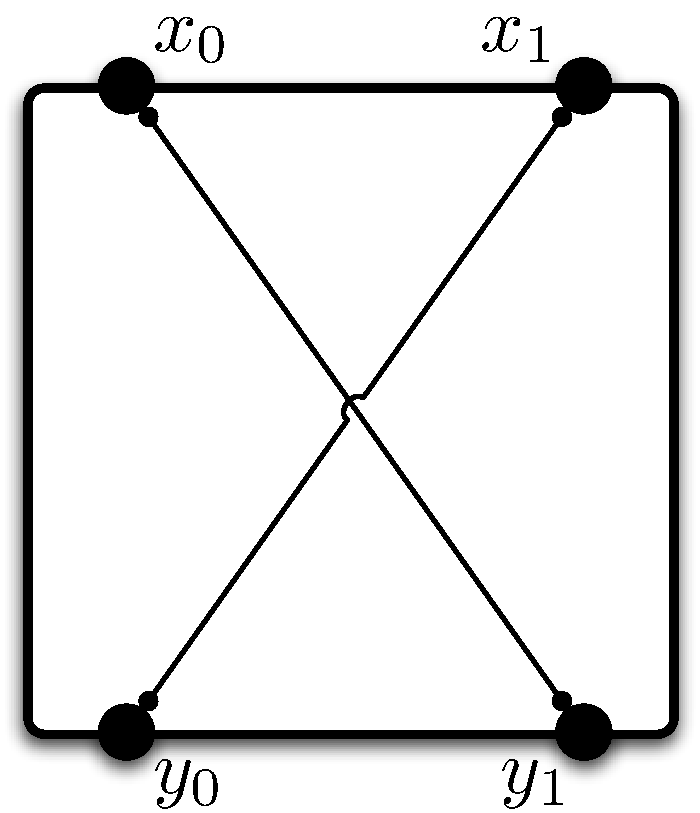
\includegraphics[viewport=0 0 390 360]{BasicCrossingCircuit.pdf}}
    %\caption{ here  }
\end{figure}
\begin{eqnarray*}
   C(x_0,x_1,y_0,y_1,u) & :=   & x_1?(s).y_0!(s).(C(x_0,x_1,y_0,y_1,u)|u!) \nonumber \\
  & & + y_0?(s).x_1!(s).(C(x_0,x_1,y_0,y_1,u)|u!) \nonumber \\
  & & + x_0?(s).u?.y_1!(s).(C(x_0,x_1,y_0,y_1,u)) \nonumber \\
  & & + y_1?(s).u?.x_0!(s).(C(x_0,x_1,y_0,y_1,u)) \nonumber
\end{eqnarray*}

A crossing process has four ports $x_0,x_1,y_0,y_1$ and a hidden
synchronizer $u$. Each port has a partner port, linked as shown in the
diagram (note the relationship to Conway's $\pm 1$ tangles
\cite{Conway1970An-enumeration-}). For example, the first behavior (indicated by the first
term of the summand) is that the process listens at port $x_1$ for a
signal $s$ (which will come, if at all, via the wiring
process). Having heard $s$, the signal is passed directly to the port
$y_0$ where the signal is then broadcast via the wiring process. Then
the process alerts the hidden synchronizer $u$ that a signal has been
passed between the ports, while concurrently preparing itself for
further signal processing. The second summand represents a signal
passing along the same strand in the opposite direction. The third and
fourth summands are similar to the first two, except that before
passing any received signal to its partner port, the process waits for
a signal from the synchronizer $u$ before allowing the signal to
pass. So the role of $u$ is that of a traffic controller who gives
priority to traffic over the route between $x_1$ and $y_0$, mimicking
an over-crossing.

\subsubsection*{Wirings}\label{sub:wirings} % (fold)

As an illustration of the expressive power of the formalism, taken
together with the short description of the calculus in the next
section, the definitions below fully equip the interested reader to
verify that wire processes are lossless, infinite capacity buffers.


\begin{eqnarray*}
    W(x,y) & := & (\nu \; n \; m)(Waiting(x,n,m) | Waiting(y,m,n)) \nonumber \\
Waiting(x,c,n) & :=   & x?(v).(\nu \; m)(Cell(n,v,m) | Waiting(x,c,m)) \nonumber \\
  & & + c?(w).c?(c).Ready(x,c,n,w) \nonumber \\
  Ready(x,c,n,w) & :=  & x?(v).(\nu \; m)(Cell(n,v,m) | Ready(x,c,m,w)) \nonumber \\
  & & + x!(w).Waiting(x,c,n) \nonumber
\end{eqnarray*}

\subsubsection*{The distinguishing power of dynamics}\label{sub:dynamic distinction} % (fold)

In summary, to each knot, $K$, the encoding $\meaningof{-}:Knots \to
\pi\textit{-calculus}$, associates an invariant, $\meaningof{K}$, an
expression in a calculus of message-passing proceses. Of note, the
notion of equivalence of knots, ambient isotopy, denoted $\sim$,
coincides perfectly with the notion of equivalence of processes,
i.e. bisimulation, denoted $\simeq$. Stated more formally,

\begin{eqnarray*}
    K_1 \sim K_2 & \iff & \meaningof{K_1} \simeq \meaningof{K_2} \nonumber
\end{eqnarray*}

(For the proof, see \cite{KnotsAsProcesses}.) In other words, unlike
other invariants, the coincidence of process dynamics with knot
characteristics enables it to be perfectly distinguishing. As dicussed
below, among the other beneficial consequences of this coincidence is
the application of process logics, especially the spatial sub-family
of the Hennessy-Milner logics, to reason about knot characteristics
and knot classes.

% subsection basic_interpretation (end)

\subsection*{The syntax and semantics of the notation system}\label{sub:the_syntax_and_semantics_of_the_notation_system} % (fold)

Having bootstrapped some intuitive account of the target calculus of
via the encoding, we summarize its technical presentation below. The
popular presentation of these calculi follows a generators and
relations style. The grammar, below, describing term constructors,
freely generates the set of processes. This set is then quotiented by
a relation known as structural congruence.

\begin{mathpar}
  \inferrule* [Left=summation] {} {{M,N} \bc \pzero \;|\; x.A \;|\; M+N}
  \and
  \inferrule* [Right=agent] {} {{A} \bc (\vec{x})P \;| \; [\vec{x}]P}
  \and \\
  \inferrule* [Left=process] {} {{P,Q} \bc N \;| \;P|Q \;| X\langle \vec{y} \rangle \;| \; (\textsf{rec} \; X(\vec{x}).P)\langle \vec{y} \rangle \;| \; (\nu \; \vec{x})P}
\end{mathpar} 

Note that the presentation uses $\vec{x}$ to denote \emph{lists} of names of
length $|\vec{x}|$. In the encodings for crossings and wires given
above we adopted the following standard abbreviations.

\begin{mathpar}
   x?(\vec{y}).P \triangleq x.(\vec{y})P \and  x!(\vec{y}).P \triangleq x.[\vec{y}]P
   \and
   X(\vec{y}) := P \triangleq (\vec{y})(\textsf{rec} \; X(\vec{x}).P)\langle \vec{y} \rangle
   \and \Pi_{i=0}^{n-1}P_i \triangleq P_0 | \ldots | P_{n-1}
\end{mathpar}

\subsection*{Structural congruence}

\begin{definition}
  The {\em structural congruence}, $\equiv$, between processes is the
  least congruence closed with respect to alpha-renaming, satisfying
  the abelian monoid laws (associativity, commutativity and $\pzero$
  as identity) for parallel composition as well as summation, and the
  following axioms:
\begin{mathpar}
 (\nu \; x)\pzero \equiv \pzero 
 \and
 (\nu \; x)(\nu \; x)P \equiv (\nu \; x)P \and (\nu \; x)(\nu \; y)P \equiv (\nu \; y)(\nu \; x)P 
 \and \\
 P | (\nu \; x)Q \equiv (\nu \; x)(P|Q), \; \mbox{\textit{if} }x \not\in \freenames{P}
 \and
 (\textsf{rec} \; X(\vec{x}).P)\langle \vec{y} \rangle \equiv P\{\vec{y}/\vec{x}\}\{(\textsf{rec} \; X(\vec{x}).P)/X\}
\end{mathpar}
\end{definition}

\subsection*{Operational semantics} 

Finally, we introduce of the computational dynamics. What marks these
algebras as distinct from other more traditionally studied algebraic
structures, e.g. vector spaces or polynomial rings, is the manner in
which dynamics is captured. In traditional structures dynamics is
expressed through morphisms between such structures, as in linear maps
between vector spaces or morphisms between rings. In algebras
associated with the semantics of computation, the dynamics is
expressed as part of the algebraic structure, itself, through a
reduction reduction relation, typically denoted by $\red$. Below we
find a recursive presentation of this relation for the calculus used
in the encoding.

\begin{mathpar}
  \inferrule* [lab=Comm] {\vec{y} \cap \vec{v} = \emptyset \\ |\vec{y}| = |\vec{z}|} { x.(\vec{y})P \juxtap x.(\nu \vec{v})[\vec{z}]P \red (\nu \vec{v})(P\{\vec{z}/\vec{y}\} | Q) }
  \and \\
  \inferrule* [lab=Par] {{P} \red {P}'} {{{P} | {Q}} \red {{P}' | {Q}}}
  \and
  \inferrule* [lab=Equiv]{{{P} \scong {P}'} \andalso {{P}' \red {Q}'} \andalso {{Q}' \scong {Q}}}{{P} \red {Q}}
  \and
  \inferrule* [lab=New] {{P} \red {P}'} {{\newp{{x}}{{P}}} \red {\newp{{x}}{{P}'}}}  
\end{mathpar}

In closing this summary, we take the opportunity to observe that it is
precisely the dynamics that differentiates this encoding. The
equivalence that coincides with ambient isotopy is a \emph{behavioral}
equivalence, i.e. an equivalence of the dynamics of processes in the
image of the encoding. In a marked departure from Gauss codes or
DT-codes or Conway's ``knotation'' this facet of the encoding affords
the \emph{conflation} of notation scheme with invariant, providing a
framework in which to establish the distinguishing power of the
invariant and a language in which to express classes of knots as
logical properties, as discussed below.

% subsection the_syntax_and_semantics_of_the_notation_system (end)   

\subsection*{Characteristic formulae}\label{sub:characteristic_formulae} % (fold)

Associated to the mobile process calculi are a family of logics known
as the Hennessy-Milner logics. These logics typically enjoy a
semantics interpreting formulae as sets of processes that when
factored through the encoding outlined above allows an identification
of classes of knots with logical formulae. In the context of this
encoding the sub-family known as the spatial logics \cite{CairesC03} \cite{Caires04} \cite{Caires04} are of particular interest providing several important
features for expressing and reasoning about properties (i.e. classes)
of knots.

\begin{description}
\item [structural connectives] The spatial logics enjoy structural
  connectives corresponding, at the logical level, to the parallel
  composition ($P | Q$) and new name ($(\nu \; x)P$) connectives for
  processes. As illustrated in the examples below, these connectives
  are extremely expressive given the shape of our encoding.
\item [decideable satisfaction] In \cite{Caires04} the satisfaction
  relation is shown to be decideable for a rich class of processes. It
  further turns out that the image of our encoding is a proper subset
  of that class. This result provides the basis for an algorithm by
  which to search for knots enjoying a given property.
\item [characteristic formulae] In the same paper, Caires presents a
  means of calculating characteristic formulae, picking out
  equivalence classes of processes up to some limit on the support set
  of names. Composed with our encoding, this characteristic formula
  can be used to pick out characteristic formulae for knots.
\end{description}

\subsubsection*{Spatial logic formulae}

The grammar below (segmented for comprehension) summarizes the syntax
of spatial logic formulae. We employ illustrative examples in the
sequel to provide an intuitive understanding of their meaning
referring the reader to \cite{Caires04} for a more detailed explication
of the semantics.

\begin{mathpar}
  \inferrule* [lab=boolean] {} {{A,B} \bc T \;|\; \neg A \;|\; A \wedge B \;|\; \eta = \eta'}
  \and
  \inferrule* [lab=spatial] {} {|\; \pzero \;|\; A | B \;|\; x \textregistered A \;|\; \forall x . A \;|\;  H x . A}
  \and
  \inferrule* [lab=behavioral] {} {|\; \alpha . A}
  \and 
  \inferrule* [lab=recursion] {} {|\; X(\vec{u}) \;|\; \mu X(\vec{u}) . A}
  \and
  \inferrule* [lab=action] {} {\alpha \bc \langle x?(\vec{y}) \rangle \;|\; \langle x!(\vec{y}) \rangle \;|\; \langle \tau \rangle}
  \and 
  \inferrule* [lab=name] {} {\eta \bc x \;|\; \tau}
\end{mathpar} 

% subsection characteristic_formulae (end)   	 

\subsection*{Example formulae}\label{sub:example_formulae_} % (fold)

\paragraph*{Crossing as formula}
\begin{mathpar}
  \textbf{C}(x0,x1,y0,y1,u) \triangleq \mu C(x0,x1,y0,y1,u).(\langle x0?(z) \rangle(\langle u! \rangle\langle y1!z \rangle C(x0,x1,y0,y1,u))
  \and \wedge \langle y1?(z) \rangle (\langle u! \rangle \langle x0!z \rangle C(x0,x1,y0,y1,u))
  \and \wedge \langle x1?(z) \rangle (\langle u? \rangle \langle y0!z \rangle C(x0,x1,y0,y1,u))
  \and \wedge \langle y0?(z) \rangle (\langle u? \rangle \langle x1!z \rangle C(x0,x1,y0,y1,u))) 
\end{mathpar}

The lexicographical similarity between shape of this formula with the
definition of the process representing a crossing reveals the
intuitive meaning of this formulae. It describes the capabilities of a
process that has the right to represent a crossing. What
differentiates the formula from the process, however, is that the
crossing process is the smallest candidate to satisfy the
formulae. Infinitely many other processes -- with internal behavior
hidden behind this interface, so to speak -- also satisfy this
formulae. Even this simple formula, then, can be seen to open a new
view onto knots, providing a computational interpretation of
\emph{virtual} knots in terms of simulation.

Note that this formula is derived by hand. A similar formula can be
derived by employing Caires calculation of characteristic formula
\cite{Caires04} to the process representing a crossing. In light of this
discussion, in the subsequent examples we let
$\meaningof{C}_{\phi}(x0,x1,y0,y1,u)$ denote a formula specifying the
dynamics we wish to capture of a crossing. To guarantee we preserve
the shape of the interface and minimal semantics we demand that
$\meaningof{C}_{\phi}(x0,x1,y0,y1,u) \Rightarrow
\textbf{C}(x0,x1,y0,y1,u)$.
                            
\paragraph*{Crossing number constraints}
Given a formula, $\meaningof{C}_{\phi}(x0,x1,y0,y1,u)$, as above we
can use the structural connectives to specify constraints on crossing
numbers, such as at least $n$ crossings, or exactly $n$ crossings.
\begin{mathpar}
  \inferrule* [lab=at-least-n] {} { K^{\geq n}_{\phi}(\vec{xs},\vec{ys}) := \Pi_{i=0}^{n-1} Hu . \meaningof{C}_{\phi}(xs_i,ys_i,u) | T }
  \and 
  \inferrule* [lab=exactly-n] {} { K^{= n}_{\phi}(\vec{xs},\vec{ys}) := \Pi_{i=0}^{n-1} Hu . \meaningof{C}_{\phi}(xs_i,ys_i,u) | \neg (\forall x_0,x_1,y_0,y_1,u . \meaningof{C}_{\phi}(x_0,x_1,y_0,y_1,u) | T) }
\end{mathpar}

To round out this section, recall that the encoding of an $n$-crossing
knot decomposes into a parallel composition of $n$ \emph{copies} of a
crossing process together with a wiring harness. To specify different
knot classes with the same crossing number amounts to specifying
logical constraints on the wiring harness. In the interest of space,
we defer examples to a forthcoming paper.

% subsection example_formulae_ (end)

% section knots_as_processes (end)

\section*{The proposed work and plan}

Three aims inform the investigation proposed here:

\begin{description}
\item [Dynamics and invariants.] Extend the well-established paradigm
  of associating algebras to topological spaces to the setting where
  the algebras hosting such invariants have dynamics – in the sense
  that they explicitly represent or embed a model of computation;
\item [Compositionality.] Exploit compositionality to expose those
  features of a space that may be analyzed locally (like the polarity
  of crossing in a knot diagram) versus those that require global
  information (like the orientation of a knot);
\item [Bisimulation.] Establish a framework in which the proof
  principle and attendant proof methods of bisimulation may be
  exported to algebraic topology.
\end{description}

\subsection*{Work to be undertaken}

The work to achieve these aims falls into three categories:

\begin{description}
\item [Theory.] Establishing the encoding is really the first step. A
  great deal of work still remains in understanding the encoding via a
  principled investigation of its connections to existing work and
  limits of applicability.
  \begin{description}
  \item [Connection to other invariants.] Current investigation
    suggests a natural correspondence to other invariants. The
    compositional nature of the encoding suggests a straightforward
    algorithm for calculating the Kauffman bracket from the process
    representation. This development warrants further research.
  \item [Knot classes as formulae.] Of special interest is tabulating
    formulae identifying a wide variety of knot classes.
  \item [Braids and links.] Further, on the knot side, because of the
    close correspondence of the basic crossing process to Conway's
    knotation primitive, it is natural to extend the encoding to links
    and braids. Initial work on the extension of the knot encoding to an encoding of links indicates a technical issue to resolve in order to implement this on the server.
  \item [Additional process calculi machinery.] On the process calculi
    side it is natural to investigate other process calculi
    (e.g. ambient calculi \cite{Cardelli04}) as possible targets. Also,
    Gardner et al.'s context logic \cite{gardner-modelling} seems particularly
    interesting as a language of properties of knots, braids and
    links.
  \end{description}
\item [Practice.] Developing the encoding to the level of robustness
  that a knot database server can be made widely accessible will also
  test the ideas and provide a potentially interesting testbed for a
  number of practical applications from biology and other physical
  sciences. This work further divides into
  \begin{description}
  \item [Efficient encoding.] To make the a practical and usable knot-search
    application it is necessary to factor the process-set semantics of
    the logic through an existing query engine. The proposal is to
    develop and prove correct an interpretation of the process-set
    semantics via XQuery, the XML query language. This interpretation
    will provide the core computation of the knot server.
  \item [Implementation.] Once developed the XQuery semantics of
    process-sets will be implemented in an XML-aware version of the
    functional language, OCaml, known as OCamlduce and a webservice
    frontend developed for handling web-based queries. Additionally,
    integration with other knot packages, especially Scharein's
    knotplot \cite{KnotPlot} will provide rendering of search results as
    graphics. Finally, a frontend domain specific language for
    expressing queries in terms of partial specifications of knots
    will be derived from the spatial logic interpretation coupled with
    the XQuery semantics.
  \end{description}
\item [Communication.] Each of these developments must be communicated
  back to the community. Being a multi-disciplinary effort the results
  span different communities (knot theorists and process algebraist)
  and as such communicating the results requires more effort because
  they must be couched in the technical languages of each field. Each
  theoretical investigation needs to be written up and published in
  peer-reviewed journals, such [JKTR] or [MSCS]. Additionally, the
  results of the practical application is also of interest to the XML
  communities and emerging webservices communities.
\end{description}

\subsection*{General plan of work}

The process by which the above objectives will be reached is now described.

The work will be carried out over a 3 year period. The project will
begin 1 September 2007 and terminate on 31 August 2010, with
deliverables expected at the end of each year. 

\begin{description}
\item [Year 1.] 
  \begin{description}
  \item [XQuery process-set semantics.] Complete specification with
    proof of correctness available as technical report.
  \item [Tabulation of knot-class formulae.] Complete specification of
    a number of distinguishing knot formulae, e.g. formulae for
    alternating knots, rational knots, toroidal knots, etc. available as technical report.
  \item [Correspondence to other invariants.] Complete specification
    and proof of correctness of the calculation of the Kauffman
    bracket from the process encodings and characteristic formulae
    available as technical report.
  \item [Comparative study of context and spatial logics.] Initial
    study of context logics versus spatial logics as a language for
    expressing properties of knots, links and braids.
  \end{description}
\item [Year 2.]
  \begin{description}
  \item [Knotserver DB: Implementation of XQuery semantics.] Working implementation of
    the XQuery interpretation of process-set semantics in OCamlduce.
  \item [Knotserver DB: Knot properties.] Working implementation of domain-specific
    language for expressing knot properties.
  \item [Knotserver DB: Webservice.] Working implementation webservice
    frontend to knot database.
  \item [Knotserver DB: Sample formulae.] Working implementation of
    knot formulae identified in first yeear expressed in domain
    specific knot property language.
  \item [Extended encoding to braids and links.] Complete specification
    of the extension of the encoding to links and braids with proof of
    theorem analogous to main theorem of \cite{KnotsAsProcesses}.
  \end{description}
\item [Year 3.]
  \begin{description}
  \item [XQuery process-set semantics.] Conference submission of XQuery
    process-set semantics.
  \item [Knotserver DB: experience.] Conference submission of
    experience paper on the construction of the knotserver db.
  \item [Tabulation of knot-class formulae.] Conference submission on
    the specification of knot properties.
  \item [Correspondence to other invariants.] Journal submission on
    the correspondence of this encoding to other knot invariants.
  \item [Comparative study of context and spatial logics.] Conference
    submission on study of context logics versus spatial logics as a
    language for expressing properties of knots, links and braids.
  \item [Extended encoding to braids and links.] Journal submission on
    the extension of the encoding to links and braids with proof of
    theorem analogous to main theorem of \cite{KnotsAsProcesses}.
  \end{description}
\end{description}

\subsection*{General personnel effort}

The PI will be devoting 25\% of the academic year and 100\% (of two
months) of each of the two summers to this project. The co-PI will be
devoting 35\% of each year to the project; the co-PI will perform the
majority of his work at his home site, Biosimilarity LLC in Seattle,
and will visit the Texas State site once per quarter during the
project. The co-PI will visit near the beginning of the project to
interact with the students. The PI and co-PI have successfully worked
together at-a-distance using a combination of e-mail, internet
messaging, and internet telephony; they will continue to do so during
this project as well, at least twice weekly.

A graduate student at the Master's level from Mathematics, will be
recruited or hired at the beginning of the project, with the aim that
they come from an underrepresented group. The graduate assistant will
be at 50\% effort. Likewise, a junior member of Biosimilarity staff
will be devoting 50\% of their time on the project for technical
support and development activities.

The high school students will attend MathWorks from late June to late
July. The co-PI will come for an extended visit during this time to
familiarize the Mathworks team with the process logics.

\subsection*{Equipment and materials}

A MacBook Pro and a MacPro is requested for the Texas State site and
two MacBook Pro's for the Biosimilarity site. The co-PI will be in
charge of directing and managing the software development. The two
nodes are needed for the co-PI to have the specific machine
architecture envisioned for serving the knots and braids
component. Instructional materials for the students will be purchased
as well.

\subsection*{Background for the educational component}

One Mathematics graduate student will participate in the
project. Ethnic minorities form 25\% of Texas State's student
body. Texas State is one of the top 20 producers of Hispanic
baccalaureate graduates in the nation. Its Mathematics Department has
a strong tradition of supporting and engaging students from
underrepresented populations. Moreover, the PI has a proven record of
accomplishment in engaging students in research projects appropriate
to their level of development.

The project will also engage a team of 2-3 high school students from
the Texas Mathworks summer program. Texas Mathworks conducts a 6-week
Honors Summer Math Camp (HSMC) for highly talented high school
students. First year students take courses in Number Theory,
Mathematica Lab, Problem Solving and an Honors Seminar. Returning
students take courses in Abstract Algebra, Analysis, and Knot
Theory. Returning students also work on research projects, mentored by
a faculty member. These projects have been outstanding, resulting in
43 Siemens-Westinghouse semi-finalists, 21 regional finalists, and 6
national finalists (2 teams) in the past 5 years. The PI will mentor
such a team, with the co-PI lending his expertise on process calculi
and Xquery (the standard extensible query language).


\newpage

\bibliographystyle{plain}   
\bibliography{../../../biblios/main.bib}


 \end{document}

